% 2. Foundations
% - [Introduction of foundations not generally known to professionals in computer science]
% - Related work [similar to respective chapters in papers: review the relevant related work by briefly summarizing it incl.used methods and achieved results, and then contrasting it with own task, i.e., show any gaps to own problem statement]


\section{Representation of Audio Signals}

In \gls{sr} systems, audio signals are typically represented as sequences of feature vectors. Various methods exist to represent these features, each providing different insights into the audio signal's characteristics and properties.

\subsection{Raw Waveform}
The raw waveform of an audio signal represents the scaled voltage amplitude of the sound wave as it varies over time. This waveform is essentially a direct digital encoding of the air pressure variations caused by sound waves. It is captured through a process of analog-to-digital conversion where the continuous sound wave is sampled at regular intervals (sampling rate) and quantized into digital values.

This representation is one of the most fundamental forms of audio data, providing a time-domain view where each sample point represents the amplitude of the audio signal at a given instant. The sampling rate, typically measured in kilohertz, defines the number of samples captured per second and is crucial in determining the quality and range of frequencies that can be accurately represented in the digital waveform.

More details on the analog-to-digital conversion process can be found in \cite{lyons2010understanding} or \cite{oppenheim1996signals}.

A raw waveform can be written as \({s} \in \mathbb{R}^l\), where \({s}[n]\) denotes the amplitude of the \(n\)-th sample, and \(l\) is the total number of samples. The sampling frequency \(f_s\), an important parameter in the analog-to-digital conversion process, dictates the temporal resolution of the waveform. The Nyquist-Shannon sampling theorem states that \(f_s\) should be at least twice the maximum frequency component present in the audio signal to adequately capture its frequency content without aliasing \cite{Nyquist1928, Shannon1949}.

In audio processing and \gls{sr} systems, the raw waveform often serves as the basis for further transformations and feature extraction methods, which transform the time-domain data into formats more suitable for various analyses and machine learning applications.

\subsection{Mel Spectogram}

Another representation method is a spectrogram, where the frequency composition ($y$-axis) of the signal is shown as it varies over time ($x$-axis). A variation of the spectrogram is the Mel spectrogram, in which each frequency of the audio signal is logarithmically scaled to better account for human perception of different frequency bands. The representation as a (Mel) spectrogram offers the advantage of a visual capture of the audio signal. Therefore, image processing models like the neural networks described in Section \ref{motivation} can be used for the algorithmic processing of audio in this representation. For the rest of this thesis, we treat the Mel spectrogram as a matrix $X$ with $M$ rows and $L$ columns, where $X[i]$ denotes the $i^{\text{th}}$ column/frame in the spectrogram:
\begin{equation}
\label{eq:spectrogram_matrixz}
    X =
    \begin{bmatrix}
    \vert & \vert & \vert & \vert & \vert &       & \vert  \\
    X[0]  & X[1]  & X[2]  & X[3]  & X[4]  &\cdots & X[L-1] \\
    \vert & \vert & \vert & \vert & \vert &       & \vert
    \end{bmatrix}
    \in \mathbb{R}^{M \times L}
\end{equation}

Figure \ref{waveform_spectrogram} shows the raw waveform of one sample of the pretraining dataset and its corresponding Mel spectrogram. More details on the conversion of time-domain signals to Mel spectrograms can be found in section \ref{sec:mel_spectrogram_conversion}.

\begin{figure}[h]
    \centering
    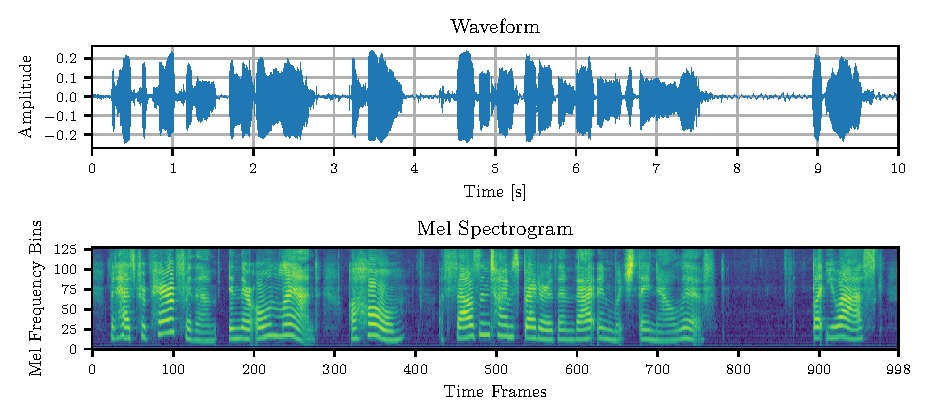
\includegraphics[width=1.0\linewidth]{img/plots/waveform_spectrogram.pdf}
    \caption{Raw waveform signal (top) and the corresponding mel spectrogram (bottom).}
    \label{waveform_spectrogram}
\end{figure}


\section{Linguistic Characteristics in the Context of Speaker Recognition}
\label{sec:spectroinformation}

To better understand the challenges in modeling prosodic features for \gls{sr}, a detailed analysis of linguistic peculiarities is required. Humans have exceptional abilities in identifying speakers and sub-tasks of \gls{sr} such as \gls{sv}. Linguistics has intensively dealt with this topic and has gained important insights. In particular, it has been shown that spectro-temporal acoustic-phonetic information is crucial for the high performance of the human brain in \gls{sr} \cites{rose2002forensic, hansen2015speaker}.

% \subsection{Spectro-temporal Acoustic-Phonetic Information in Language}\label{sec:spectroinformation}
% 1 subsectin wo die einzig isch inere section sött mer glaub vermide

\textit{Spectro-temporal acoustic-phonetic information} refers to the combination of spectral (frequency-related) and temporal (time-related) properties of speech signals. Spectral information includes the distribution of energy across various frequency bands of the speech signal. This can be used to identify features such as formants, which represent characteristic resonance frequencies in human speech. Formants manifest as peaks in the spectrum and enable the identification of characteristic frequency patterns associated with certain vowels \cite{small1998phonetics}. This is shown in Figure~\ref{fig:formants}.

\begin{figure}[h]
\begin{subfigure}[b]{0.47\textwidth}
   \centering
   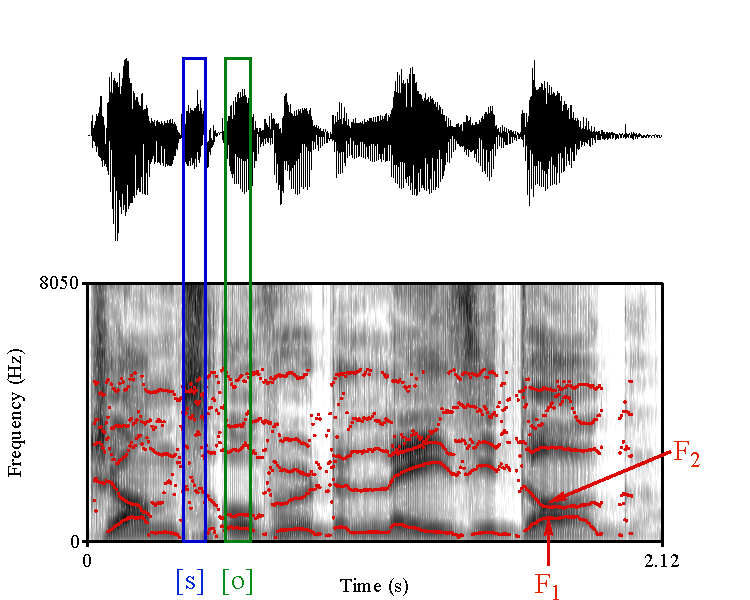
\includegraphics[width=1\textwidth]{img/english-sound-segment-nice3.pdf}
\end{subfigure}%
\begin{subfigure}[b]{0.53\textwidth}
   \centering
   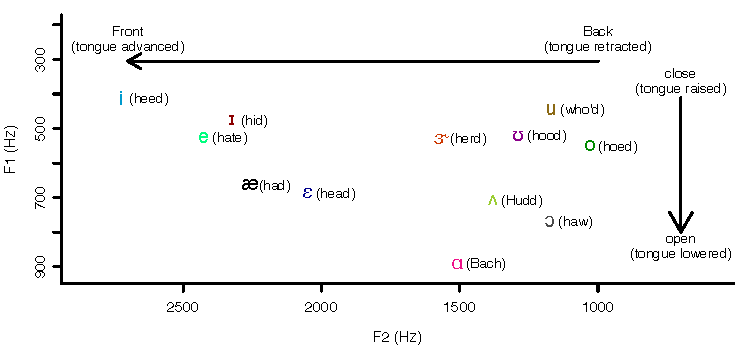
\includegraphics[width=1\textwidth]{img/AllvowelsH95--formants-raw--mean.pdf}
\end{subfigure}
\caption{Raw waveform and corresponding spectrogram of a speech recording (left); average vowel formants in the $F_1,F_2$ vowel space over a set of 139 speakers (right). Image from \cite{tavakoli2024statistics}.}
\label{fig:formants}
\end{figure}

Temporal information refers to the sequence of sound events in the speech signal, characterized by features such as stress patterns, speaking rate, and intonation patterns. Stress patterns describe the emphasis of certain syllables, while speaking rate indicates the number of sounds or words per unit of time. Intonation describes the melody and pitch of the language.

The combination of these spectral and temporal information allows for the capture and analysis of complex linguistic features, which is crucial for automatic speech recognition, speech synthesis, and other speech processing applications. In phonetics, it is generally recognized that these features are unique and can thus be assigned to an individual speaker.


\section{Audio Signal Processing Using DNNs}

The basic approach to \gls{sr} using \glspl{dnn} is works as follows.
The voice recording is transformed into a suitable format. Often, this is a Mel spectrogram, as information not relevant to human perception is filtered out from the audio signal. This reduction in information content can be justified because humans excel in \gls{sr}, thus the audio information perceivable by the human auditory organ should also be sufficient for a \gls{dnn}.

% \subsection{Frame-based Acoustic Information - \gls{fba}}

The audio signal is then divided into overlapping time windows, which serve as input for the \gls{dnn}. These windows typically have a length in the range of several tens of milliseconds. This approach offers several advantages: By using segments of the audio signal, the amount of data is reduced, leading to simpler models with lower dimensionality and shorter training time. Moreover, this method makes the model more robust against environmental noise, as it learns local features. These local features contain, as described in section \ref{sec:spectroinformation}, spectral information \gls{fba}. However, research points out that \gls{sst} plays a significant role in human \gls{sr} \cite{stadelmann2009unfolding}. To what extent \gls{dnn} consider \gls{sst} is discussed in \cite{neururer2023deep}.

\section{Quantifying the Utilization of SST}
\label{foundation_sst}

The mentioned paper, \cite{neururer2023deep}, represents the first systematic approach to investigate the modeling of \gls{sst} in \gls{dnn}. This section explains the method developed by the authors, which forms the basis and motivation for the present work.

The goal is to investigate whether state-of-the-art \gls{dnn}, when removing the \gls{sst} from the spectrogram inputs, are still able to achieve good performance in \gls{sr} tasks. If this is the case, it can at least be argued that \gls{dnn} are capable of compensating for the loss of \gls{sst} and therefore do not necessarily rely on them, but can instead rely on the remaining \gls{fba}.

To remove the \gls{sst} from the spectrogram while preserving the \gls{fba}, two approaches have been pursued:
\vspace{-\parskip}
\begin{itemize}[topsep=0.5\parskip, itemsep=0.0\parskip, parsep=0.5\parskip]
    \item \textbf{\gls{ss}}: The spectrogram is divided into equal-sized segments, within which the data is swapped on the time axis. %\glsunset{ss}
    \item \textbf{\gls{su}}: The spectrogram is also divided into equal-sized segments, but the data is swapped on the time axis before segmenting. %\glsunset{su}
\end{itemize}

Figure \ref{shuffle_sst_exploitation} illustrates the described process of swapping spectrogram information.

\begin{figure}[H]
\centering
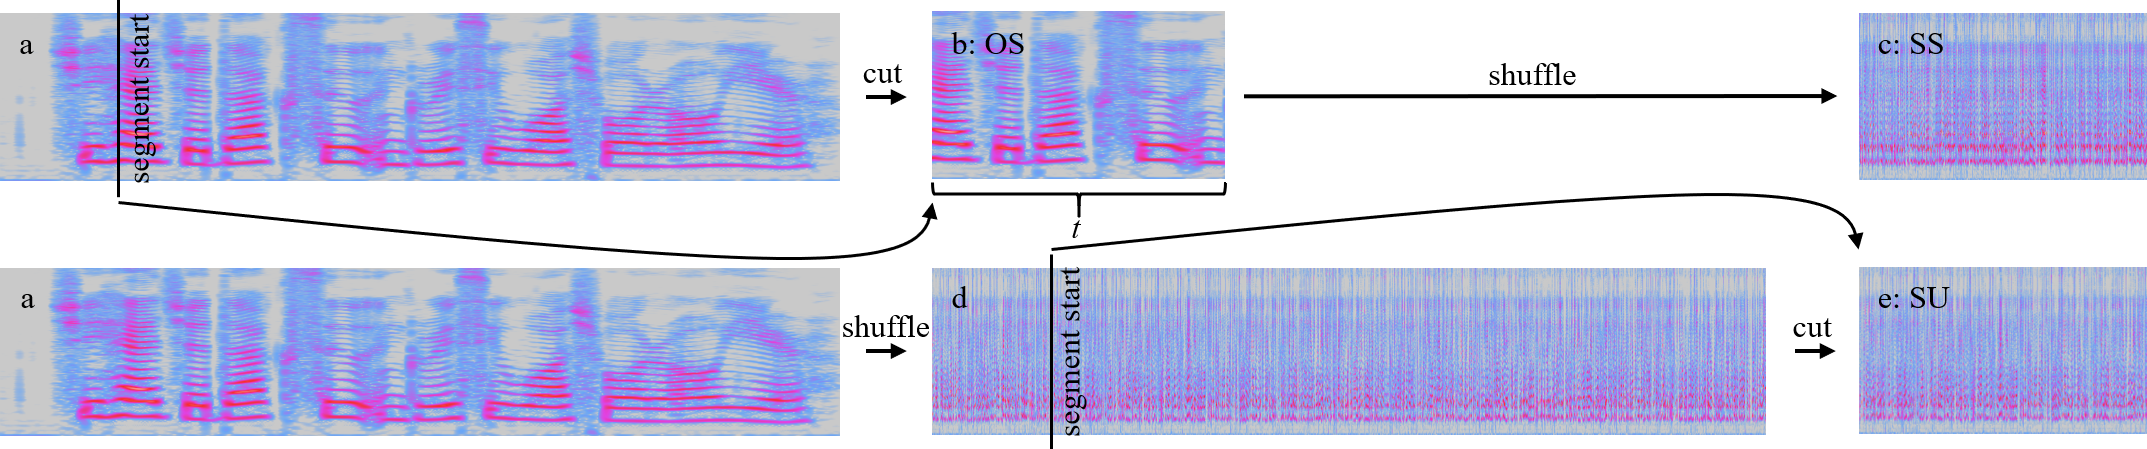
\includegraphics[width=1.0\linewidth]{img/segment-drawing.png}
\caption{Generation and shuffling of segments (image from \cite{neururer2023deep}).}
\label{shuffle_sst_exploitation}
\end{figure}

In \cite{neururer2023deep}, various \gls{dnn} models for \gls{sr} are tested on different training and evaluation datasets. This includes training on \gls{os} and evaluation on \gls{os}, \gls{ss}, and \gls{su} as well as training on \gls{ss} and evaluation on \gls{os}, \gls{ss}, and \gls{su}, and training on \gls{su} and evaluation on \gls{os}, \gls{ss}, and \gls{su}. The evaluated architectures include a \gls{cnn}, a \gls{rnn}, a \gls{resnet} and the F-\gls{resnet}. The results of these experiments are shown in Table \ref{sst_exploitation_results}.

In particular, the results show that training and evaluation on swapped data (SS/SS and SU/SU) deliver state-of-the-art performance in \gls{sc} and \gls{sv}, although the model does not utilize \gls{sst}. These results cast significant doubts on whether \glspl{dnn} actually learn \gls{sst} or whether they rely exclusively on \gls{fba} features \cite{neururer2023deep}.

If the performance of training and evaluation on the shuffled data were significantly lower than the performance of training and evaluation on the original data, it could be stated that the model relies on both \gls{fba} and \gls{sst}. 

The present thesis therefore investigates the performance of Transformers in \gls{sv} tasks and tries to determine whether they rely on \gls{sst}.

\newcommand{\OrigSeg}{OS}
\newcommand{\ShuffleSeg}{SS}
\newcommand{\ShuffleUtterance}{SU}

\newcommand{\markcell}[1]{\scriptsize{#1}$\Downarrow$\footnotesize}
\setlength{\tabcolsep}{2pt} % for the horizontal padding

\begin{table}[H]
	\centering
     \caption{Test results as reported in \cite{neururer2023deep} using original and shuffled spectrograms from the TIMIT dataset using four different \glspl{dnn}. \Gls{sc} performance (left) is measured using the \gls{mr} ($\mu/\sigma$) and \gls{sv} performance (right) is measured using the \gls{eer} ($\mu/\sigma$). Bold font indicates best results per model, cell coloring scales with quality per model.}
    %\begin{adjustbox}{width=\textwidth}
    	\begin{tabular}{ll|rrr|rrr}
    		\hline
    	 \multicolumn{2}{c|}{task $\rightarrow$}
    		 & \multicolumn{3}{c|}{Speaker Clustering}
    		 & \multicolumn{3}{c}{Speaker Verification} \\

    		 \multicolumn{2}{c|}{\scriptsize{training $\downarrow$ / test $\rightarrow$}}
    		 & \multicolumn{1}{c}{\OrigSeg}
    		 & \multicolumn{1}{c}{\ShuffleUtterance}
    		 & \multicolumn{1}{c|}{\ShuffleSeg}
    		 & \multicolumn{1}{c}{\OrigSeg}
    		 & \multicolumn{1}{c}{\ShuffleUtterance}
    		 & \multicolumn{1}{c}{\ShuffleSeg} \\ 
            \hline
    		\multirow{3}{*}{CNN \cite{lukic2017learning}}
    		 & \OrigSeg
    		 & \cellcolor[RGB]{0, 255, 0} \textbf{0.00 \scriptsize{$\sigma$0.00}}
    		 & \cellcolor[RGB]{255, 0, 0} 9.75 \scriptsize{$\sigma$0.94}
    		 & \cellcolor[RGB]{255, 39, 0} 9.00 \scriptsize{$\sigma$2.15}
    		 & \cellcolor[RGB]{80, 255, 0} 6.38 \scriptsize{$\sigma$0.12}
    		 & \cellcolor[RGB]{255, 0, 0} 12.02 \scriptsize{$\sigma$0.51}
    		 & \cellcolor[RGB]{255, 9, 0} 11.90 \scriptsize{$\sigma$0.46} \\
    		 & \ShuffleUtterance
    		 & \cellcolor[RGB]{255, 65, 0} 8.50 \scriptsize{$\sigma$2.42}
    		 & \cellcolor[RGB]{26, 255, 0} 0.50 \scriptsize{$\sigma$0.61}
    		 & \cellcolor[RGB]{91, 255, 0} 1.75 \scriptsize{$\sigma$0.61}
    		 & \cellcolor[RGB]{245, 255, 0} 8.55 \scriptsize{$\sigma$0.49}
    		 & \cellcolor[RGB]{16, 255, 0} 5.55 \scriptsize{$\sigma$0.06}
    		 & \cellcolor[RGB]{60, 255, 0} 6.12 \scriptsize{$\sigma$0.12} \\
    		 & \ShuffleSeg
    		 & \cellcolor[RGB]{255, 39, 0} 9.00 \scriptsize{$\sigma$1.66}
    		 & \cellcolor[RGB]{52, 255, 0} 1.00 \scriptsize{$\sigma$0.50}
    		 & \cellcolor[RGB]{65, 255, 0} 1.25 \scriptsize{$\sigma$0.00}
    		 & \cellcolor[RGB]{215, 255, 0} 8.16 \scriptsize{$\sigma$0.42}
    		 & \cellcolor[RGB]{0, 255, 0} \textbf{5.33 \scriptsize{$\sigma$0.18}}
    		 & \cellcolor[RGB]{34, 255, 0} 5.78 \scriptsize{$\sigma$0.16} \\
    		\hline
    		\multirow{3}{*}{RNN \cite{stadelmann2018capturing}}
    		 & \OrigSeg
    		 & \cellcolor[RGB]{170, 255, 0} 1.25 \scriptsize{$\sigma$1.12}
    		 & \cellcolor[RGB]{255, 136, 0} 2.75 \scriptsize{$\sigma$0.94}
    		 & \cellcolor[RGB]{255, 135, 0} 2.75 \scriptsize{$\sigma$0.50}
    		 & \cellcolor[RGB]{0, 255, 0} \textbf{3.53 \scriptsize{$\sigma$0.07}}
    		 & \cellcolor[RGB]{255, 0, 0} 4.19 \scriptsize{$\sigma$0.09}
    		 & \cellcolor[RGB]{255, 224, 0} 3.90 \scriptsize{$\sigma$0.12} \\
    		 & \ShuffleUtterance
    		 & \cellcolor[RGB]{255, 0, 0} 3.75 \scriptsize{$\sigma$1.37}
    		 & \cellcolor[RGB]{0, 255, 0} \textbf{0.00 \scriptsize{$\sigma$0.00}}
    		 & \cellcolor[RGB]{255, 169, 0} 2.50 \scriptsize{$\sigma$1.58}
    		 & \cellcolor[RGB]{255, 149, 0} 3.99 \scriptsize{$\sigma$0.16}
    		 & \cellcolor[RGB]{189, 255, 0} 3.78 \scriptsize{$\sigma$0.10}
    		 & \cellcolor[RGB]{97, 255, 0} 3.66 \scriptsize{$\sigma$0.13} \\
    		 & \ShuffleSeg
    		 & \cellcolor[RGB]{255, 238, 0} 2.00 \scriptsize{$\sigma$1.00}
    		 & \cellcolor[RGB]{170, 255, 0} 1.25 \scriptsize{$\sigma$0.79}
    		 & \cellcolor[RGB]{33, 255, 0} 0.25 \scriptsize{$\sigma$0.50}
    		 & \cellcolor[RGB]{255, 144, 0} 4.00 \scriptsize{$\sigma$0.07}
    		 & \cellcolor[RGB]{255, 232, 0} 3.89 \scriptsize{$\sigma$0.06}
    		 & \cellcolor[RGB]{4, 255, 0} 3.54 \scriptsize{$\sigma$0.05} \\
    		\hline
    		\multirow{3}{*}{ResNet \cite{xie2019utterance}}
    		 & \OrigSeg
    		 & \cellcolor[RGB]{0, 255, 0} \textbf{1.00 \scriptsize{$\sigma$0.94}}
    		 & \cellcolor[RGB]{255, 157, 0} 8.25 \scriptsize{$\sigma$4.78}
    		 & \cellcolor[RGB]{255, 0, 0} 11.50 \scriptsize{$\sigma$4.29}
    		 & \cellcolor[RGB]{0, 255, 0} \textbf{4.96 \scriptsize{$\sigma$0.19}}
    		 & \cellcolor[RGB]{255, 0, 0} 10.34 \scriptsize{$\sigma$1.56}
    		 & \cellcolor[RGB]{255, 106, 0} 9.21 \scriptsize{$\sigma$1.15} \\
    		 & \ShuffleUtterance
    		 & \cellcolor[RGB]{72, 255, 0} 2.50 \scriptsize{$\sigma$1.77}
    		 & \cellcolor[RGB]{0, 255, 0} \textbf{1.00 \scriptsize{$\sigma$0.50}}
    		 & \cellcolor[RGB]{97, 255, 0} 3.00 \scriptsize{$\sigma$1.27}
    		 & \cellcolor[RGB]{154, 255, 0} 6.59 \scriptsize{$\sigma$0.25}
    		 & \cellcolor[RGB]{122, 255, 0} 6.25 \scriptsize{$\sigma$0.23}
    		 & \cellcolor[RGB]{133, 255, 0} 6.37 \scriptsize{$\sigma$0.35} \\
    		 & \ShuffleSeg
    		 & \cellcolor[RGB]{84, 255, 0} 2.75 \scriptsize{$\sigma$0.94}
    		 & \cellcolor[RGB]{12, 255, 0} 1.25 \scriptsize{$\sigma$1.12}
    		 & \cellcolor[RGB]{0, 255, 0} \textbf{1.00 \scriptsize{$\sigma$0.94}}
    		 & \cellcolor[RGB]{87, 255, 0} 5.89 \scriptsize{$\sigma$0.25}
    		 & \cellcolor[RGB]{108, 255, 0} 6.11 \scriptsize{$\sigma$0.31}
    		 & \cellcolor[RGB]{79, 255, 0} 5.80 \scriptsize{$\sigma$0.11} \\
    		\hline
    		\multirow{3}{*}{F-ResNet \cite{chung2020in}}
    		 & \OrigSeg
    		 & \cellcolor[RGB]{117, 255, 0} 11.50 \scriptsize{$\sigma$2.15}
    		 & \cellcolor[RGB]{255, 0, 0} 37.50 \scriptsize{$\sigma$4.18}
    		 & \cellcolor[RGB]{255, 57, 0} 33.75 \scriptsize{$\sigma$4.18}
    		 & \cellcolor[RGB]{114, 255, 0} 12.20 \scriptsize{$\sigma$0.25}
    		 & \cellcolor[RGB]{255, 0, 0} 23.41 \scriptsize{$\sigma$1.73}
    		 & \cellcolor[RGB]{255, 104, 0} 20.47 \scriptsize{$\sigma$1.50} \\
    		 & \ShuffleUtterance
    		 & \cellcolor[RGB]{192, 255, 0} 16.50 \scriptsize{$\sigma$2.42}
    		 & \cellcolor[RGB]{30, 255, 0} 5.75 \scriptsize{$\sigma$1.70}
    		 & \cellcolor[RGB]{7, 255, 0} 4.25 \scriptsize{$\sigma$1.00}
    		 & \cellcolor[RGB]{217, 255, 0} 15.12 \scriptsize{$\sigma$0.84}
    		 & \cellcolor[RGB]{53, 255, 0} 10.46 \scriptsize{$\sigma$0.28}
    		 & \cellcolor[RGB]{26, 255, 0} 9.69 \scriptsize{$\sigma$0.20} \\
    		 & \ShuffleSeg
    		 & \cellcolor[RGB]{178, 255, 0} 15.50 \scriptsize{$\sigma$2.57}
    		 & \cellcolor[RGB]{45, 255, 0} 6.75 \scriptsize{$\sigma$1.50}
    		 & \cellcolor[RGB]{0, 255, 0} \textbf{3.75 \scriptsize{$\sigma$0.79}}
    		 & \cellcolor[RGB]{246, 255, 0} 15.91 \scriptsize{$\sigma$0.90}
    		 & \cellcolor[RGB]{32, 255, 0} 9.86 \scriptsize{$\sigma$0.11}
    		 & \cellcolor[RGB]{0, 255, 0} \textbf{8.95 \scriptsize{$\sigma$0.13}} \\
    		\hline
    	\end{tabular}
    %\end{adjustbox}
    \label{sst_exploitation_results}
\end{table}


\section{Contrastive Loss}
Contrastive loss is a metric learning technique widely used in machine learning to measure the similarity between pairs of data points. The idea of contrastive loss is to ensure that similar data points (positive pairs) are closer in an embedding space, while dissimilar data points (negative pairs) are farther apart. 

Contrastive loss was introduced in the context of Siamese networks, where the goal is to learn a function that maps input data into an embedding space where the similarity between data points can be easily measured \cite{Hadsell2006DimensionalityRB}. For \gls{sv}, it means that intra-speaker embeddings are closer in the embedding space while inter-speaker embeddings are farther apart. The contrastive loss function is described in \ref{methods_contrastive_loss}.



















% \section{Sprachliche Besonderheiten im Kontext der Sprechererkennung}

% Um die Herausforderungen bei der Modellierung prosodischer Merkmale für die Sprechererkennung (SV) besser zu verstehen, ist eine eingehende Analyse der Sprachbesonderheiten erforderlich. Der Mensch verfügt über außergewöhnliche Fähigkeiten bei der Identifizierung von Sprechern und deren Teilaufgaben wie der Sprecherüberprüfung (Speaker Verification). Die Linguistik hat sich intensiv mit dieser Thematik befasst und dabei wichtige Erkenntnisse gewonnen. Insbesondere hat sich gezeigt, dass spektro-temporale akustisch-phonetische Informationen für die hohe Leistungsfähigkeit des menschlichen Gehirns in der Sprechererkennung entscheidend sind \cites{rose2002forensic, hansen2015speaker}.

% \subsection{Spektro-temporale akustisch-phonetische Informationen in der Sprache}\label{sec:spectroinformation}

% \textit{Spektro-zeitliche akustisch-phonetische Informationen} beziehen sich auf die Kombination spektraler (frequenzbezogener) und zeitlicher Eigenschaften von Sprachsignalen. Spektrale Informationen umfassen die Verteilung der Energie in verschiedenen Frequenzbereichen des Sprachsignals. Diese können zur Identifizierung von Merkmalen wie Formanten genutzt werden, die charakteristische Resonanzfrequenzen in der menschlichen Sprache repräsentieren. Formanten manifestieren sich als Peaks im Spektrum und ermöglichen die Identifizierung charakteristischer Resonanzfrequenzen, die bestimmten Vokalen zugeordnet werden können \cite{small1998phonetics}.

% Zeitliche Informationen beziehen sich auf die Abfolge von Schallereignissen im Sprachsignal, die durch Merkmale wie Betonungsmuster (Stress Pattern), Sprechgeschwindigkeit (Speaking Rate) und Intonationsmuster gekennzeichnet sind. Betonungsmuster beschreiben die Hervorhebung bestimmter Silben, während die Sprechgeschwindigkeit die Anzahl von Lauten oder Wörtern pro Zeiteinheit angibt. Die Intonation beschreibt die Melodie und Tonhöhe der Sprache.

% Die Kombination dieser spektralen und zeitlichen Informationen ermöglicht die Erfassung und Analyse komplexer sprachlicher Merkmale, was für automatische Spracherkennung, Sprachsynthese und andere sprachverarbeitende Anwendungen von entscheidender Bedeutung ist. In der Linguistik wird allgemein anerkannt, dass diese Merkmale eindeutig sind und somit einem individuellen Sprecher zugeordnet werden können.

% \section{Representation of audio signals}

% In Sprechererkennungsalgorithmen werden Audiosignale in der Regel als Merkmalsvektoren repräsentiert. Es existieren verschiedene Methoden zur Darstellung dieser Merkmale.

% \subsection{Waveform}

% In einem Waveform wird die Amplitute über die Zeit dargestellt. 

% \subsection{Mel Spectogram}

% Eine weitere Darstellungsmethode ist das Mel-Spektrogramm, bei dem jede Frequenz des Audiosignals in Bezug zu ihrer Amplitude logarithmisch skaliert wird, um die menschliche Wahrnehmung unterschiedlicher Frequenzbänder besser zu berücksichtigen.

% Diese Darstellungen bieten den Vorteil einer visuellen Erfassung des Audiosignals. Daher können auch Bildverarbeitungsmodelle wie die in Abschnitt 1.1 beschriebenen neuronalen Netzwerke für die algorithmische Verarbeitung von Audiosignalen herangezogen werden. Dieser Ansatz repräsentiert den aktuellen Stand der Technik für Sprechererkennungssysteme und erzielt beeindruckende Ergebnisse.

% \section{Audiosignal Verarbeitung mithilfe von \gls{dnn}}

% Die grundsätzliche Vorgehensweise der Sprechererkennung mithilfe von \gls{dnn} ist vereinfacht dargestellt wie folgt.
% Die Sprachaufnahme wird in ein geignetes Format transformiert. Häufig ist dies ein Mel Spektogram, da Informationen, welche nicht für die menschliche Wahrnehmung relevant sind, aus dem Audiosignal ausgefiltert werden. Diese Reduktion des Informationsgehaltes kann damit begründet werden, dass der Mensch in der Sprechererkennung absolut briliert und somit die Audioinformationen, welche für das menschliche Hörorgan wahrnehmbar sind, für ein \gls{dnn} ausreichend sein müssen.

% \subsection{Frame-based acoustic information - \gls{fba}}

% Das Audiosignal wird dann in überlappende Zeitfenster unterteilt, die als Eingabe für das \gls{dnn} dienen. Diese Fenster haben üblicherweise eine Länge im Bereich von einigen zehn Millisekunden. Dieser Ansatz bietet verschiedene Vorteile: Durch die Verwendung von Ausschnitten des Audiosignals wird die Datenmenge reduziert, was zu simpleren Modellen mit geringerer Dimensionalität führt und die Trainingszeit verkürzt. Darüber hinaus macht diese Methode das Modell robuster gegenüber Umgebungsgeräuschen, da es lokale Merkmale lernt. Diese lokalen Merkmale enthalten, wie in Abschnitt \ref{sec:spectroinformation} beschrieben, spektrale Informationen \gls{fba}. Linguisten weisen jedoch auch darauf hin, dass die beschriebenen segmentalen zeitlichen Informationen \gls{sst} eine bedeutende Rolle in der Sprechererkennung spielen \cite{neururer2023deep}. In wie weit Modelle \gls{sst} berücksichtigen wird wird in folgendem Paper beschrieben\cite{neururer2023deep}. 

% \section{Quantifizierung der SST-Ausnutzung}

% Die vorliegende Studie von Neururer, Dellwo und Stadelmann ("Deep Neural Networks for Automatic Speaker Recognition Do Not Learn Supra-Segmental Temporal Features") stellt einen erstmaligen systematischen Ansatz zur Diskussion, der sich mit der Modellierung supra-segmentaler zeitlicher Merkmale (\gls{sst}) durch Deep Neural Networks (\gls{dnn}) befasst. Dieser Abschnitt dient der Erläuterung dieses Ansatzes, der als Grundlage und Motivation für die vorliegende Arbeit dient.

% Ziel ist es, zu untersuchen, ob State-of-the-Art \gls{dnn} bei der Entfernung der \gls{sst} aus den Spektrogrammeingaben weiterhin gute Leistungen bei Sprechererkennungsaufgaben (\gls{sr}) erzielen können. Falls dies der Fall ist, kann zumindest argumentiert werden, dass \gls{dnn} in der Lage sind, den Verlust von \gls{sst} zu kompensieren und daher nicht zwingend darauf angewiesen sind, sondern sich stattdessen auf die verbleibenden frame-basierten akustischen Merkmale (\gls{fba}) stützen können.

% Zur Entfernung der \gls{sst} aus dem Spektrogramm und gleichzeitig zur Erhaltung der \gls{fba} können zwei Ansätze verfolgt werden:

%     \textbf{SS-Ansatz}: Das Spektrogramm wird in gleich große Segmente unterteilt, innerhalb derer die Daten auf der Zeitachse vertauscht werden.

%     \textbf{SU-Ansatz}: Das Spektrogramm wird ebenfalls in gleich große Segmente unterteilt, jedoch werden die Daten vor der Segmentierung auf der Zeitachse vertauscht.

% Die nachfolgende Abbildung veranschaulicht den beschriebenen Vorgang des Vertauschens der Spektrogramminformationen.

% \begin{figure}[h]
%     \centering
%     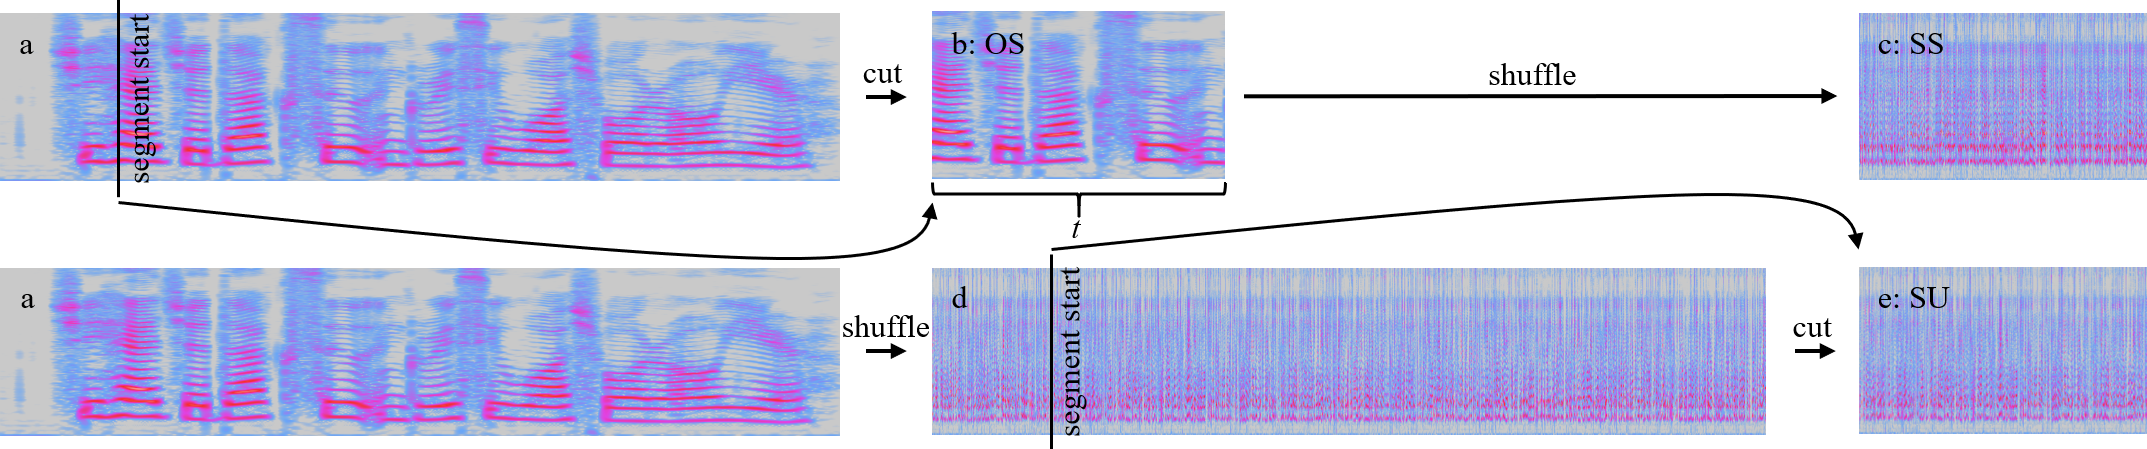
\includegraphics[width=1.0\linewidth]{img/segment-drawing.png}
%     \caption{Erzeugung und Vertauschung von Segmenten (adaptiert von \cite{neururer2023deep}).}
%     \label{shuffle_sst_exploitation}
% \end{figure}

% In der genannten Studie werden verschiedene \gls{dnn}-Modelle für Sprechererkennung (\gls{sv}) und -verifizierung (\gls{sc}) auf unterschiedlichen Trainings- und Auswertungsdatensätzen getestet. Dies umfasst das Training auf den originalen Segmenten (OS) und die Auswertung auf OS, SS und SU sowie das Training auf SS und die Auswertung auf OS, SS und SU und das Training auf SU und die Auswertung auf OS, SS und SU. Die Ergebnisse sind in der folgenden Grafik dargestellt.

% \begin{figure}[h]
%     \centering
%     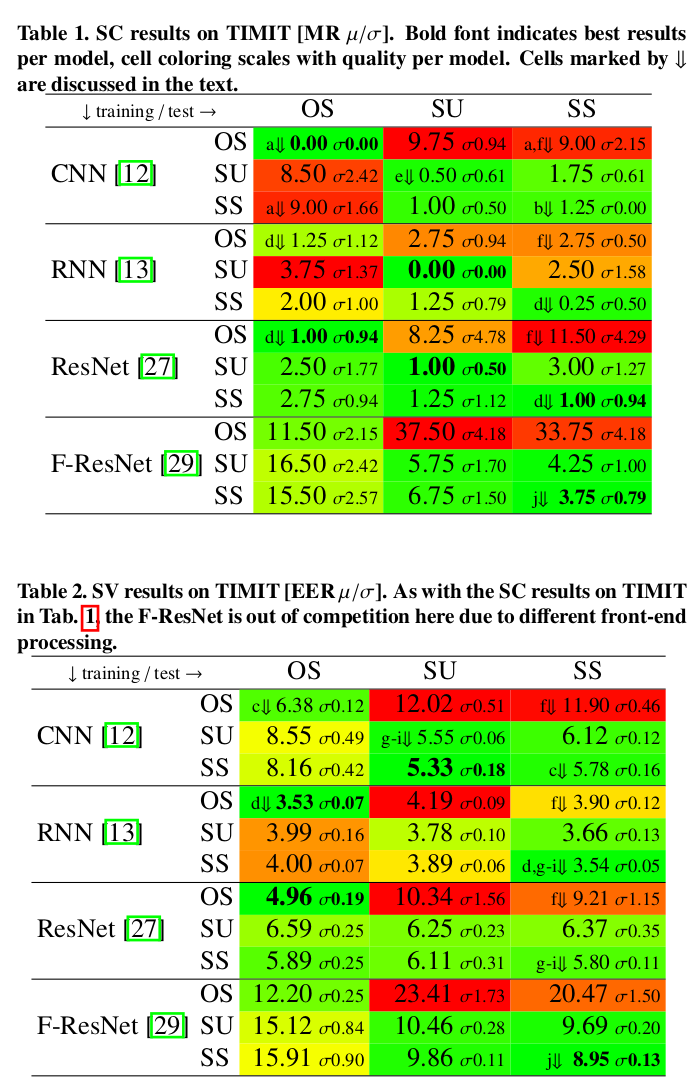
\includegraphics[width=0.54\linewidth]{img/neururer_resultate.png}
%     \caption{Testergebnisse von \gls{sc} und \gls{sv} unter Verwendung von originalen und vertauschten Segmenten (adaptiert von \cite{neururer2023deep}).}
%     \label{sst_exploitation_results}
% \end{figure}


% Insbesondere zeigt sich aus den Ergebnissen, dass das Training und die Auswertung auf vertauschten Daten (SS/SS und SU/SU) State-of-the-Art-Leistungen in \gls{sc} und \gls{sv} liefern, obwohl das Modell keine \gls{sst} nutzt. Diese Ergebnisse werfen erhebliche Zweifel darüber auf, ob \gls{dnn} überhaupt \gls{sst} erlernen oder ob sie sich ausschließlich auf \gls{fba}-Merkmale verlassen \cite{neururer2023deep}.

% Falls die Performance von Training und Evaluation auf den geshuffelten Daten signifikant tiefer als die Performance von Training und Evaluation auf den originalen Daten ist, so kann ausgesagt werden, dass das Model sowohl auf die \gls{fba} als auch \gls{sst} angewiesen ist. Die vorliegende Arbeit untersucht daher die Performance von Transformer Netzwerken in \gls{sv} Tasks und versucht festzustellen, ob Transformer Netzwerke auf \gls{sst} angewiesen sind. 










